\subsubsection{Módulo NFC}

Permite que se seleccionen canciones y emisoras mediante el móvil con NFC.


Los ficheros más destacables del módulo son:

\begin{enumerate}
	\item \texttt{nfc.c}: Hilo que gestiona el uso de la tag. Los datos obtenidos se envían por una cola al hilo de control.
	\item \texttt{nfc.h}: Exporta la función para el arranque del hilo.
\end{enumerate}

El principal problema a la hora de utilizar este componente, es que no pueden estar activos al mismo tiempo, por lo que hemos tenido que adaptar la utilización de estos dos protocolos con el uso real de nuestro módulo NFC. A la hora de guardar y leer datos, en ambos casos, se guardan en NDEF. 

Nosotros vamos a utilizar RF mediante el uso del teléfono móvil para escribir en el NDEF, mientras que el I2C para leer el contenido, por lo que solo contaremos con esos uso. Para escribir mediante RF, la tranferencia consiste en dos pulsos a nivel bajo en el GPO. 

Por esto mismo, el código consiste en habilitar el RF (DIS = 0), esperar a una subida en el GPO y esperar 500 ms (Asegurando que se ha completado la transferencia). Después, se deshabilita el RF (DIS = 1) y se procede a enviar todas las transmisiones por I2C. Finalmente, se envía la información al hilo de control y se procede a habilitar de nuevo el RF y volver a esperar al flanco de subida.

A la hora de trabajar con el I2C, utilizaremos la familia de comandos NFC Forum Type 4 Tag, mientras que con RF se utiliza ISO/IEC 7816-4. En lo referente a I2C, tenemos que crear las tramas correspondientes a cada comando. Nosotros utilizaremos:

\begin{enumerate}
\item NDEF Tag Application Select: Selecciona la aplicación NDEF Tag.
\item NDEF Select: Selecciona el fichero NDEF.
\item Read Binary: Lee datos de un fichero.
\end{enumerate}

Los utilizaremos de la siguiente manera:

\begin{figure}[h]
    \centering
    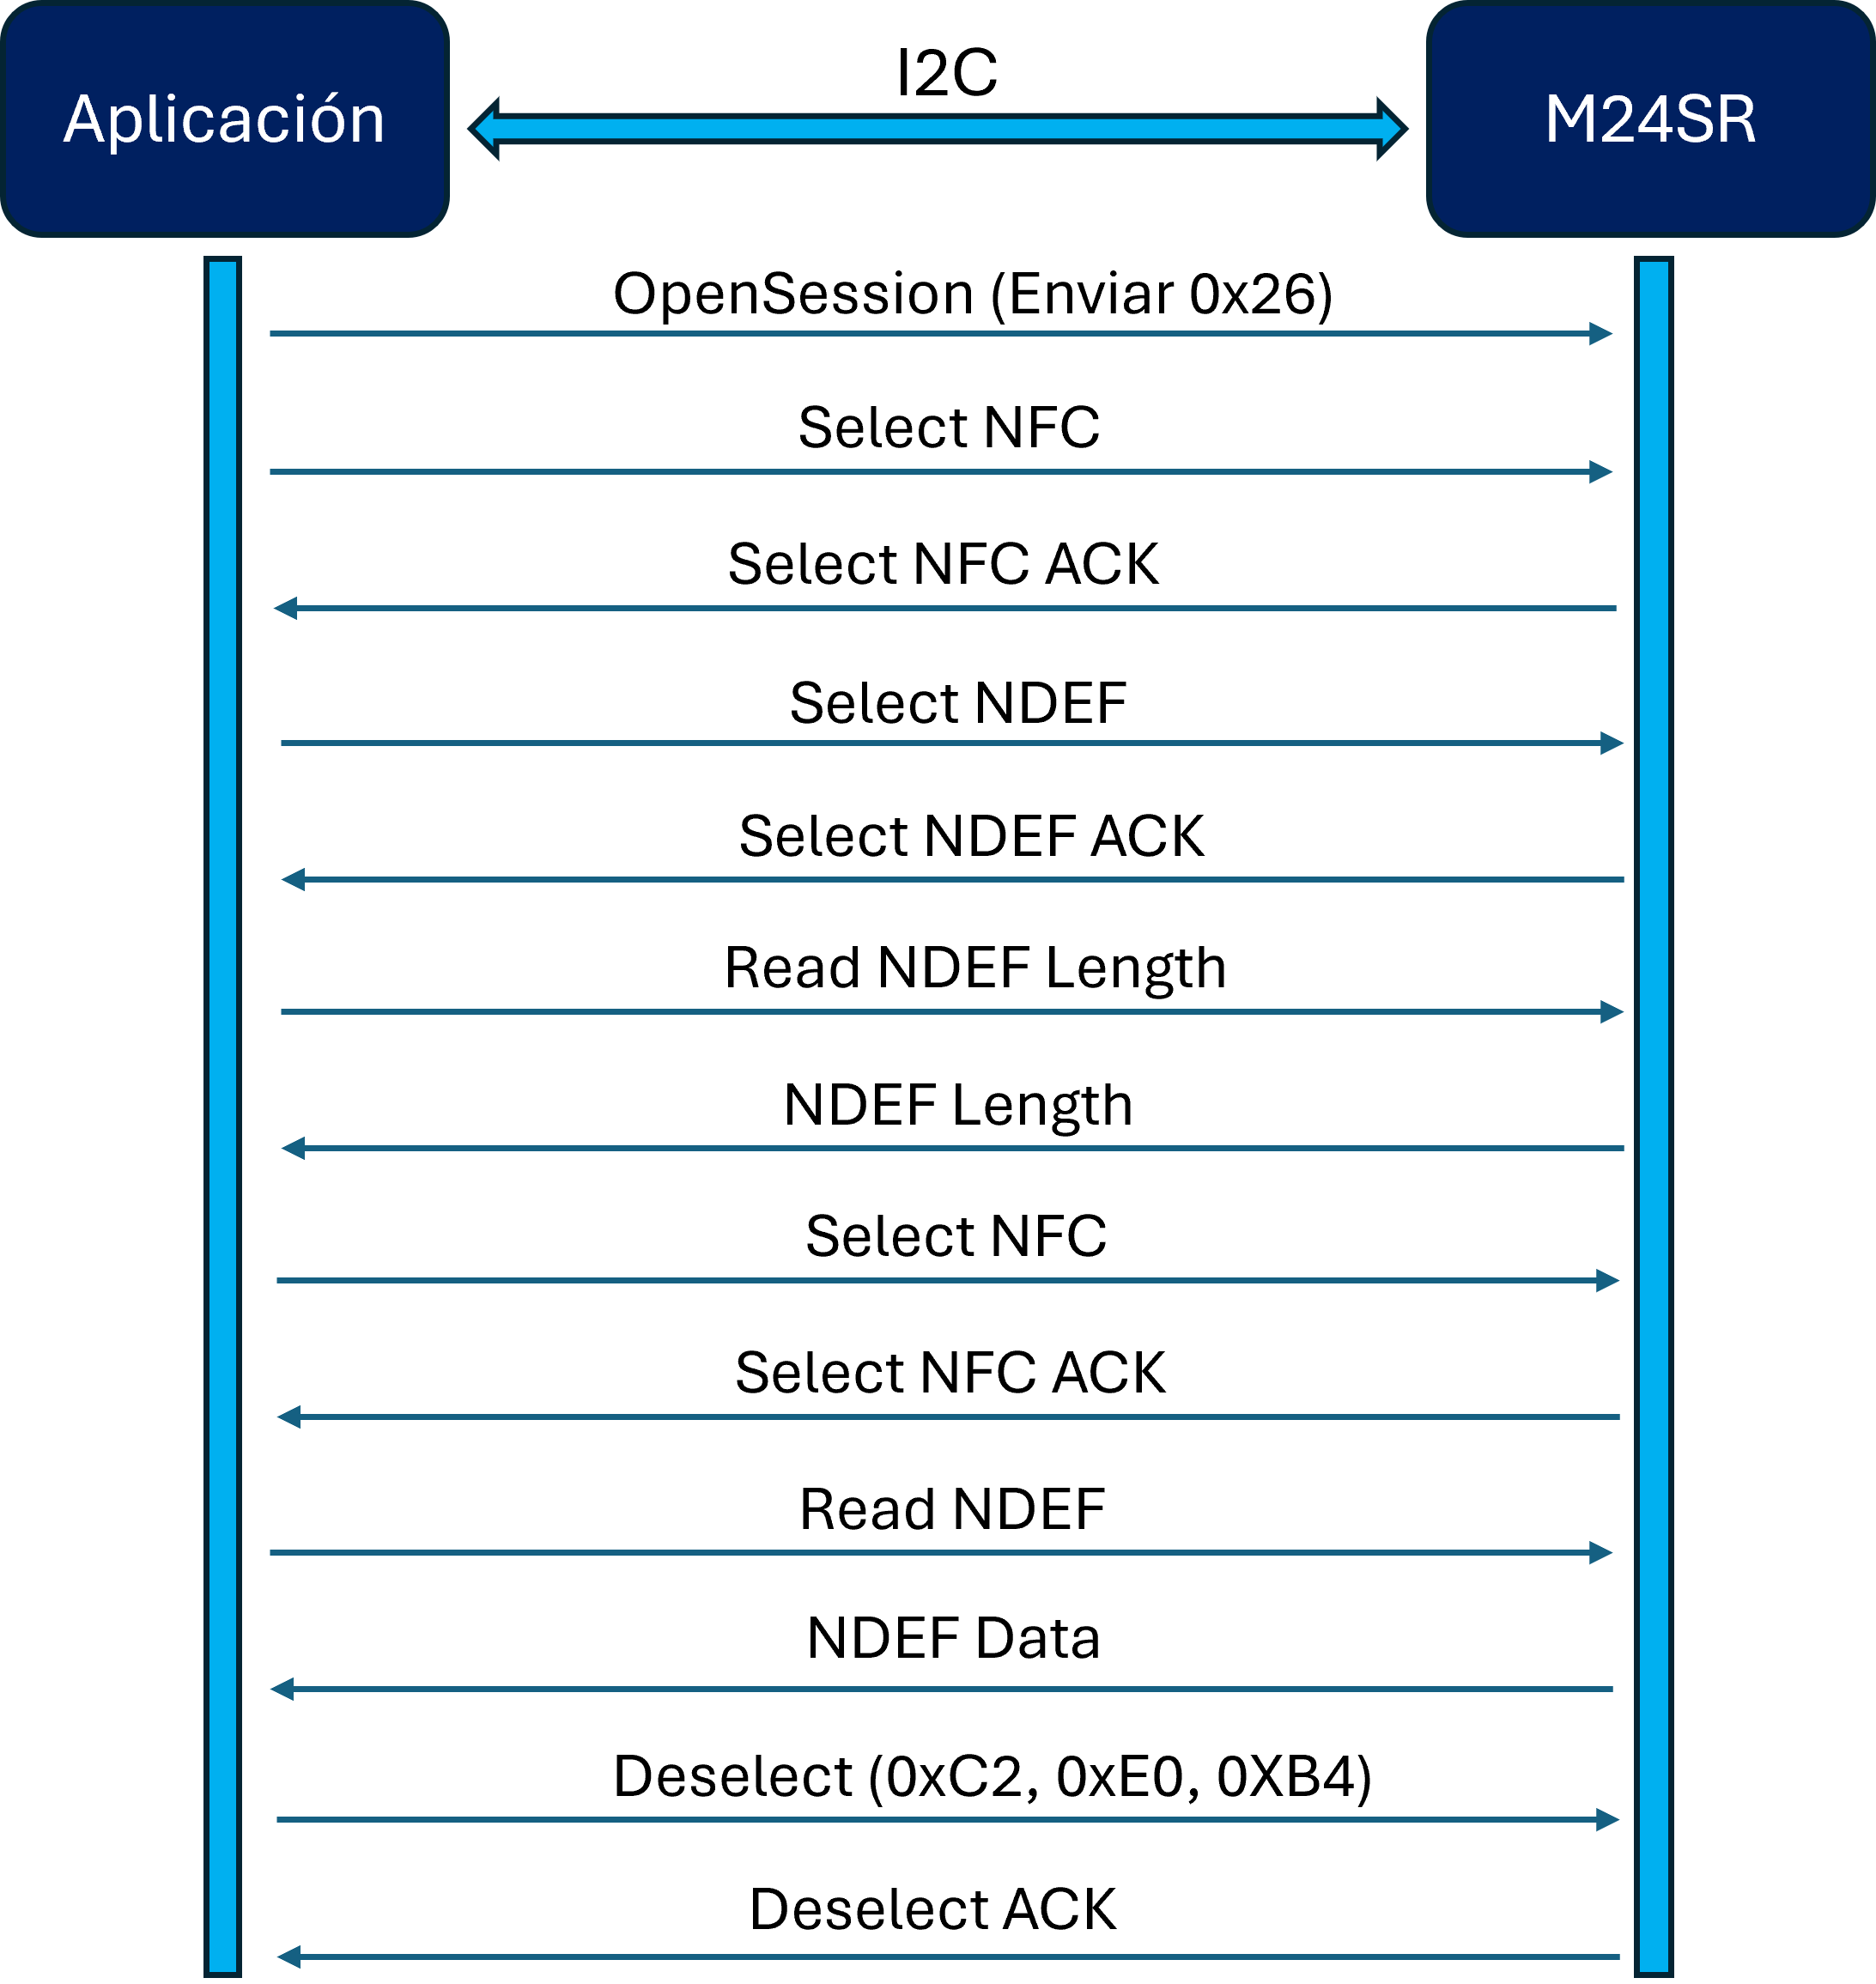
\includegraphics[width=0.5\textwidth]{images/3/3-2/SD/Diagrama.png}
    \caption{Diagrama de flujo de una operación de lectura con el NFC}
    \label{fig:label}
\end{figure}

Todos los bytes para las transferencias los hemos calculado gracias al datasheet del componente M24SR64-Y. Además, antes de enviar el master recieve, hay que esperar por los tiempos de la tarjeta (\texttt{osDelay(5)}).

El módulo también utiliza CRC para la detección de errores en transferencias I2C. Cada byte I2C se calcula utilizando ese algoritmo, y al final de la trama se envían 2 bytes con el valor calculado. Para cacularlo, hemos utilizado la siguiente página web \cite{CalculoCRC}, introduciendo todos los bytes de la trama.

Los mensajes que hemos definido para el NFC están compuestos por una letra ('S' = canción, 'R' = radio) y 4 números (Nº canción o emisora de radio).

Ejemplos: 
	- \texttt{S 0014}: Se quiere escuchar la canción nº 14.
	- \texttt{R 1029}: Se quiere escuchar la emisora 102.9 FM.